\section{Theorie}
\label{sec:Theorie}
Im Inneren eines Metalls herrscht näherungsweise ein konstantes, positives Potential, welches um den Wert $\phi$
von dem der äußeren Umgebung abweicht. Dadurch wirken im Inneren eines Metalls keine Kräfte auf die darin 
befindlichen Elektronen, wodurch sie sich, wie Moleküle eines Gases, frei bewegen können. Um aus der Metalloberfläche
auszutreten, muss allerdings ein Potential $\xi $ überwunden werden, indem die materialspezifische Austrittsarbeit
$ e_0\xi$ aufgebracht wird. Dies ist durch ein Potentialtopf-Modell zu veranschaulichen, welches in  \ref{fig:pottopf}
gezeigt ist. 
 \begin{figure}
     \centering
     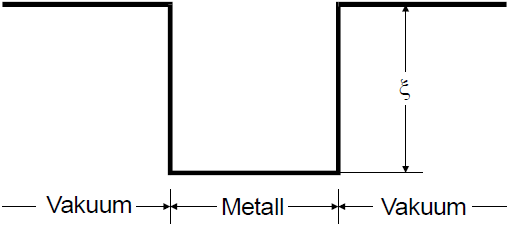
\includegraphics[height=4cm]{data/pottopf.png}
     \caption{Potentialtopf-Modell für Elektronen im Metall}
     \label{fig:pottopf}
 \end{figure}
\FloatBarrier
Die Möglichkeit, dass Elektronen die Metalloberfläche spontan verlassen, ist nur über die Quantentheorie zu beantworten.
Zum einen kann ein Elektron nur diskrete Energiewerte annehmen. Außerdem kann nach dem Pauli-Verbot ein bestimmter Energiezustand $E$ nur von zwei 
Elektronen, die jeweils entgegengesetzten Spin haben, gleichzeitig angenommen werden. Anders als in der klassischen Statistik muss also ein Elektron
auch für $T=0$ eine Energie, die ungleich null ist, besitzen. Die maximale Energie in diesem Zustand wird durch die Fermische Grenzenergie $\zeta$
beschrieben, die von der Elektronendichte im Metall abhängt. 
Die Fermi-Diracsche Verteilungsfunktion
\begin{equation}
    f(E) = \frac{1}{exp \Bigl(\frac{E-\zeta}{kT}\Bigr) +1}
\end{equation}

beschreibt die Wahrscheinlichkeit für einen Energiezustand, von einem Elektron eingenommen zu werden. 
Sie kann für Elektronen mit hinreichend großer Energie durch 
\begin{equation}
    f(E) \approx exp \Bigl(\frac{\zeta-E}{kT}\Bigr)
\end{equation} angenähert werden. Die Abbildung \ref{fig:fermi} zeigt die Wahrscheinlichkeiten für unterschiedliche Werte $E$, sowohl bei 
$T=0$, als auch bei $T \gg 0$.
\begin{figure}
    \centering
    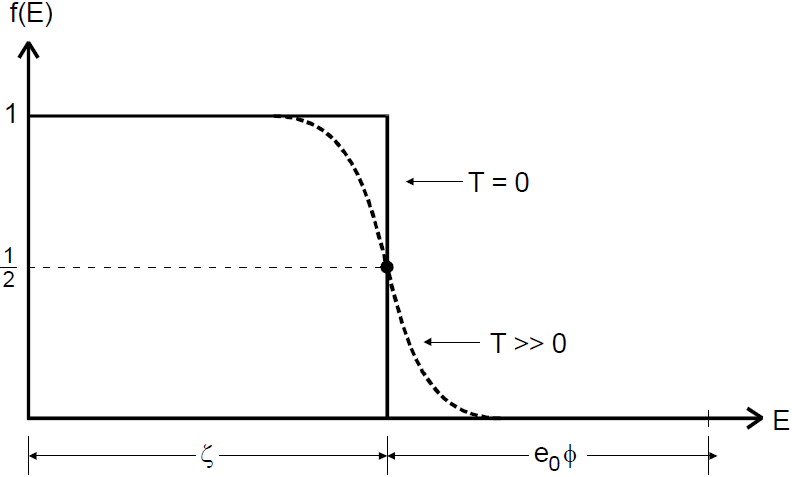
\includegraphics[height=5cm]{data/fermi.png}
    \caption{Wahrscheinlichkeitsverteilung der Energiezustände}
    \label{fig:fermi}
\end{figure}
\FloatBarrier
Die Zahl $n(E)$ der Elektronen pro Volumeneinheit des Phasenraumes lässt sich dabei durch 
\begin{equation}
    n(E) = \frac{2}{h^3} f(E)
\end{equation}  
beschreiben, wobei $h$ das Planksche Wirkungsquantum angibt. Letztendlich lässt sich die Sättigungsstromdichte $j_S(T)$ über die sogenannte
Richardson-Gleichung 
\begin{equation}
    j_S(T) = 4\pi \frac{e_0 m_0 k^2 T^2}{h^3} exp\Bigl(\frac{-e_0 \phi}{kT}\Bigr)
    \label{eqn:richard}
\end{equation}
berechnen. 
\\
Für die Messung eines Sättigungstromes ist die Verwendung einer Hochvakuum-Diode notwendig. Innerhalb dieser herrscht ein Vakumm, welches 
garantiert, dass keine Wechselwirkungen zwischen den freigesetzten Elektronen und den Gasmolukälen der Luft passieren können. Außerdem ist 
eine Saugspannung zwischen der Glühkathode und einer Anode angeschlossen, wodurch die freigesetzten Elektronen in Richtung der Anode beschleunigt
werden. Der schematische Aufbau ist der Abbildung \ref{fig:diode} dargestellt.
\begin{figure}
    \centering
    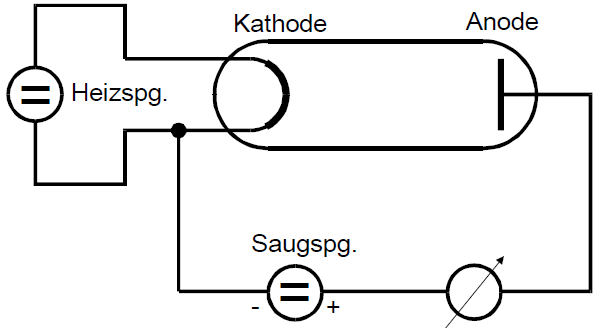
\includegraphics[height=5cm]{data/aufbau.png}
    \caption{Schmatischer Aufbau der Hochvakuumdiode}
    \label{fig:diode}
\end{figure}
\FloatBarrier
Um einen rein von der Kathodentemperatur abhängigen Anodenstrom zu beobachten, muss die Anodenspannung hinreichend groß sein. Vor Erreichen dieses 
Wertes ist allerdings auch das Ohmsche Gesetzt ungültig, da die Elektronen keine konstante Geschwindigkeit in Richtung der Anode haben, sondern 
zu dieser hin beschleunigt werden. Damit ist die Raumladungsdichte $\rho$ ortsabhängig und nimmt zur Anode hin ab. Da sich $\rho$ auf die 
Feldstärke zwischen Kathode und Anode auswirkt, bzw. das Feld der Kathode abschirmt, kommen nicht alle emittierten Elektronen an der Anode an,
wodurch der gemessene Diodenstrom kleiner als der erwartete Sättigungstrom ist. Über das Langmuir-Schottkysche Ramladungsgesetz lässt sich ein 
Zusammenhang zwischen der Stromdichte $j$ und der Anodenspannung $V$ herstellen. Damit gilt 
\begin{equation}
    j = \frac{4}9 \epsilon_0 \sqrt{2e_0/m_0} \frac{V^{\frac{3}2}}{a^2}\,
    \label{eqn:langmuir}
\end{equation}
dessen Gültigkeit sich auf das sogenannte Raumladungsgebiet beschränkt. Folglich müsste theoretisch bei $V=0$ auch $j=0$ sein. Allerdings 
ist bei $V=0$ noch ein Anodenstrom zu beobachten, der aufgrund der Eigengeschwindigkeit der Elektronen bestehen bleibt. Einige Elektronen 
können dadurch sogar gegen eine Gegenspannung anlaufen. Der so enstehende Strom wird Anlaufstrom genannt. In Abbildung \ref{fig:anlauf} sind 
die Energieverhällnisse zwischen Kathode und Anode im Anlaufstromgebiet dargestellt. 
\begin{figure}
    \centering
    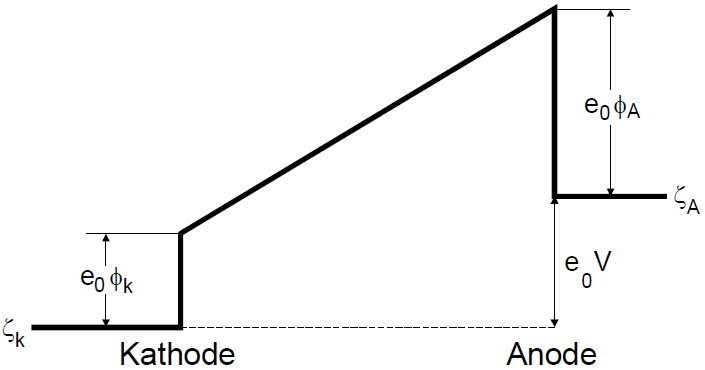
\includegraphics[height=4cm]{data/potdiff.png}
    \caption{Potentialdifferenz im Anlaufstromgebiet}
    \label{fig:anlauf}
\end{figure}
\FloatBarrier

Die Kennlinie der Diode beschreibt einen Zusammenhang zwischen der Stromdichte $j$ und dem angelegten Potential. Die drei charakteristischen 
Gebiete sind das Anlaufstromgebiet, das Raumladungsgebiet und das Sättigungstromgebiet. Im Anlaufstromgebiet für $V < 0$ steigt der Anodenstrom
exponentiell, während die daran anschließende Steigung innerhalb des Raumladungsgebietes eine $\sqrt{V^3}$-Abhängigkeit hat. Schließlich geht 
im Sättigungstromgebiet der Anodenstrom asymptotisch gegen den Sättigungstrom $I_S$.
Aus einer solchen Kennlinie können die Kathodentemperatur und die Austrittsarbeit bestimmt werden.
Die Kathodentemperatur kann über den Zusammenhang 
\begin{equation}
    T_f U_f = f \eta \sigma T^4 + N_\text{WL} 
\end{equation} 
ermittelt werden. Dabei ist $f$ die emittierende Kathodenoberfläche, $\sigma$ die Stefan-Boltzmannsche Strahlungskonstante, $\eta$ der 
Emissionsgrad der Oberfläche und $N_\text{WL} $ die Wärmeleistung. 
Ein Beispiel für den Verlauf einer Kennlinie zeigt die 
Abbildung \ref{fig:kennlinie}. 
\begin{figure}
    \centering
    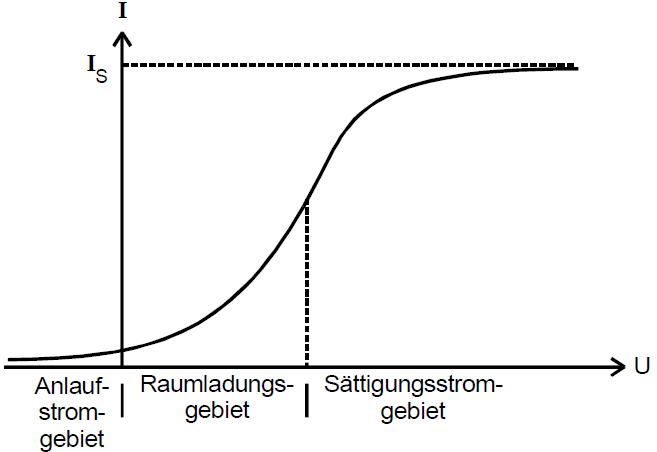
\includegraphics[height=6cm]{data/kennlinie.png}
    \caption{Kennlinie der Hochvakuumdiode}
    \label{fig:kennlinie}
\end{figure}
\FloatBarrier

